\documentclass[a4paper,10pt]{article}
\usepackage{amsmath}
\usepackage{graphicx}
\usepackage{color}

% If you want to use Chinese, include the following package
\usepackage{CJKutf8}

\title{CS532100 Numerical Optimization Homework 1}
\author{Student ID Name}
\date{Due Nov 11}
\begin{document}
\maketitle
\begin{enumerate}
 \item (45\%) Consider a function $f(x_1,x_2) = x_1^3x_2-2x_1x_2^2+x_1x_2^3$. 
    \begin{enumerate}
    \item Compute the gradient and Hessian of $f$.
    \item Is $(x_1,x_2)=(1,1)$ a local minimizer? Justify your answer.
    \item What is the steepest descent direction of $f$ at $(x_1, x_2) = (1, 2)$?
    \item What is the Newton's direction of $f$ at $(x_1,x_2)=(1,2)$?
    \item Compute the LDL decomposition of the Hessian of $f$ at $(x_1,x_2)=(1,2)$. (No pivoting)
    \item Is the Newton's direction of $f$ at $(x_1, x_2) = (1, 2)$ a descent direction? Justify your answer.
    \item Modify the LDL decomposition computed in (d) such that
all diagonal elements of $D$ is larger than or equal to 1, and use
the modified LDL decomposition to compute a modified Newton’s
direction at $(x_1, x_2) = (1, 2)$.
    \item Suppose $\vec{x_0} = (1, 1)$ and $\vec{x_1} = (1, 2)$ and $B_0 = I$, compute the quasi Newton direction $p_1$ using SR1.
    \item Suppose $\vec{x_0} = (1, 1)$ and $\vec{x_1} = (1, 2)$ and $B_0 = I$, compute the quasi Newton direction $p_1$ using BFGS. 
    \end{enumerate}
    
{\color{blue} Answers are put here. 

\begin{CJK*}{UTF8}{bsmi}
$\\$可以用中文作答。
\end{CJK*}
}

\item (20\%) 
    \begin{enumerate}
    \item A set $S\subseteq R^n$ is a $\emph{convex}$ set if the straight line connecting any two points in $S$ is also entirely in $S$.  
    A function $f:S\rightarrow R$ is a $\emph{convex}$ function if $S$ is a convex set. The following properties are equivalent:
        \begin{enumerate}
            \item $S\subseteq R^n$ is a convex set, $f:S\rightarrow R$ is a convex function.
            \item $f(\alpha\vec{x}+(1-\alpha)\vec{y})\leq\alpha f(\vec{x})+(1-\alpha)f(\vec{y})$ for all $\alpha\in [0, 1]$, $\vec{x}, \vec{y}\in S$.
        \end{enumerate}
        Prove that when $f$ is a convex function, any local minimizer $\vec{x}^\ast$ is a global minimizer of $f$.
        $\\$(Hint: Suppose there is another point $\vec{z}\in S$ such that $f(\vec{z})\leq f(\vec{x}^\ast)$, then $\vec{x}^\ast$ is not a local minimizer.)
        \item Suppose $f(\vec{x}) = \vec{x}^T Q\vec{x}$ , where $Q$ is a symmetric positive semidefinite matrix, show that $f(\vec{x})$ is a convex function.$\\$
        (Hint: It might be easier to show $f(\vec{y}+\alpha(\vec{x}-\vec{y}))-\alpha f(\vec{x}) - (1-\alpha)f(\vec{y})\leq 0$.)
    \end{enumerate}

{\color{blue} Answers are put here. 

\begin{CJK*}{UTF8}{bsmi}
$\\$可以用中文作答。
\end{CJK*}

}

\item (20\%) (Line search method) Suppose $\phi(\alpha) = f(\vec{x_k} + \alpha\vec{p_k}) = (\alpha - 1)^2$.
    \begin{enumerate}
        \item The sufficient decrease condition asks $\phi(\alpha)\leq\phi(0)+c_1\alpha\phi'(0),\\ \alpha\in[0,\infty)$.
        Suppose $c_1 = 0.1$, what is the feasible interval of $\alpha$ satisfying this condition ?
        \item The curvature condition asks $\phi'(\alpha)\geq c_2\phi'(0)$. 
        Suppose $c_2 = 0.9$, what is the feasible interval of $\alpha$ satisfying this condition ?
    \end{enumerate}
    
{\color{blue} Answers are put here.

\begin{CJK*}{UTF8}{bsmi}
$\\$可以用中文作答。
\end{CJK*}

}



\item (15\%) The conjugate gradient method for solving $Ax=b$ is given in Figure 1, where $z_k$ is the approximate solution. 
In class we only showed that $\alpha_k = (\vec{p_k}^T\vec{r_k})/(\vec{p_k}^T A\vec{p_k})$ and $\beta_k = -(\vec{p_k}^T A\vec{r_{k+1}})/(\vec{p_k}^T A\vec{p_k})$. 
Prove that the above formula of $\alpha_k$ and $\beta_k$ are equivalent to the ones in step (3) and step (6). 
You may need the relations in step (4) and step (5), and the following properties:
    \begin{enumerate}
        \item $\vec{r_i}^T\vec{r_j} = 0$ for all $i\neq j$.
        \item $\vec{p_i}^TA\vec{p_j} = 0$ for all $i\neq j$.
        \item $\vec{p_k}$ is a linear combination of $\vec{r_0},....\vec{r_k}$, $\vec{p_k} = \sum_{i=1}^k \gamma_i\vec{r_i}$.
        $\\$(which can be shown from step (7) by mathematical induction. )
    \end{enumerate}
\begin{figure}[h]
\centering
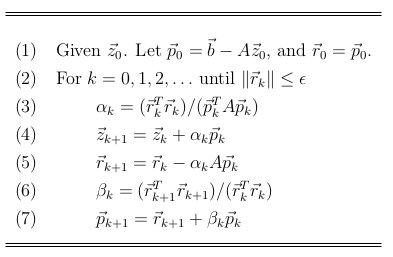
\includegraphics[scale=0.75]{Figure 1.png}
\caption{The CG algorithm.}
\label{fig1}
\end{figure}
{\color{blue} Answers are put here.

\begin{CJK*}{UTF8}{bsmi}
$\\$可以用中文作答。
\end{CJK*}
}


\end{enumerate}

\end{document}
